% 
% Annual Cognitive Science Conference
% Sample LaTeX Paper -- Proceedings Format
% 

% Original : Ashwin Ram (ashwin@cc.gatech.edu)       04/01/1994
% Modified : Johanna Moore (jmoore@cs.pitt.edu)      03/17/1995
% Modified : David Noelle (noelle@ucsd.edu)          03/15/1996
% Modified : Pat Langley (langley@cs.stanford.edu)   01/26/1997
% Latex2e corrections by Ramin Charles Nakisa        01/28/1997 
% Modified : Tina Eliassi-Rad (eliassi@cs.wisc.edu)  01/31/1998
% Modified : Trisha Yannuzzi (trisha@ircs.upenn.edu) 12/28/1999 (in process)
% Modified : Mary Ellen Foster (M.E.Foster@ed.ac.uk) 12/11/2000
% Modified : Ken Forbus                              01/23/2004
% Modified : Eli M. Silk (esilk@pitt.edu)            05/24/2005
% Modified : Niels Taatgen (taatgen@cmu.edu)         10/24/2006
% Modified : David Noelle (dnoelle@ucmerced.edu)     11/19/2014
% Modified : Roger Levy (rplevy@mit.edu)     12/31/2018



%% Change "letterpaper" in the following line to "a4paper" if you must.

\documentclass[10pt,letterpaper]{article}

\usepackage{cogsci}
\usepackage{pslatex}
\usepackage{apacite}
\usepackage{float} % Roger Levy added this and changed figure/table
                   % placement to [H] for conformity to Word template,
                   % though floating tables and figures to top is
                   % still generally recommended!
                   
%\cogscifinalcopy % Uncomment this line for the final submission 


%\usepackage[none]{hyphenat} % Sometimes it can be useful to turn off
%hyphenation for purposes such as spell checking of the resulting
%PDF.  Uncomment this block to turn off hyphenation.

\usepackage{graphicx}
\usepackage{amsmath}
\usepackage{xcolor}

\newcommand{\tableref}[1]{Table~\ref{#1}}
\newcommand{\figref}[1]{Figure~\ref{#1}}
\newcommand{\expref}[1]{Experiment~#1}

%\setlength\titlebox{4.5cm}
% You can expand the titlebox if you need extra space
% to show all the authors. Please do not make the titlebox
% smaller than 4.5cm (the original size).
%%If you do, we reserve the right to require you to change it back in
%%the camera-ready version, which could interfere with the timely
%%appearance of your paper in the Proceedings.

\definecolor{Red}{RGB}{180,20,140}
\newcommand{\jd}[1]{\textcolor{Red}{\textbf{[jd: #1]}}} 

\title{Replicating eye-tracking research using incremental decision tasks and web-based libraries} 
 
\author{{\large \bf Judith Degen (jdegen@stanford.edu)} \\
  Department of Psychology, 1202 W. Johnson Street \\
  Madison, WI 53706 USA
  \AND {\large \bf Leyla Kursat (lkursat@stanford.edu)} \\
  Department of Educational Psychology, 1025 W. Johnson Street \\
  Madison, WI 53706 USA}


\begin{document}

\maketitle


\begin{abstract}

\jd{write}

\textbf{Keywords:} 
psycholinguistics; experimental pragmatics;  scalar implicature; linking functions; eye-tracking
\end{abstract}


\section{Introduction}

\jd{include general linking function refs (see qing et al refs and also newer stuff by jim magnuson)}

\jd{include linking function for xprag refs: qing et al, jasbi et al, franke 2014 and franke newer paper (see our scil paper), scontras, waldon and degen}

\section{Sun \& Breheny (2020) -- the original experiment}

We replicate \expref{3} of \citeA{sun2020}.

\begin{figure}[H]
\centering
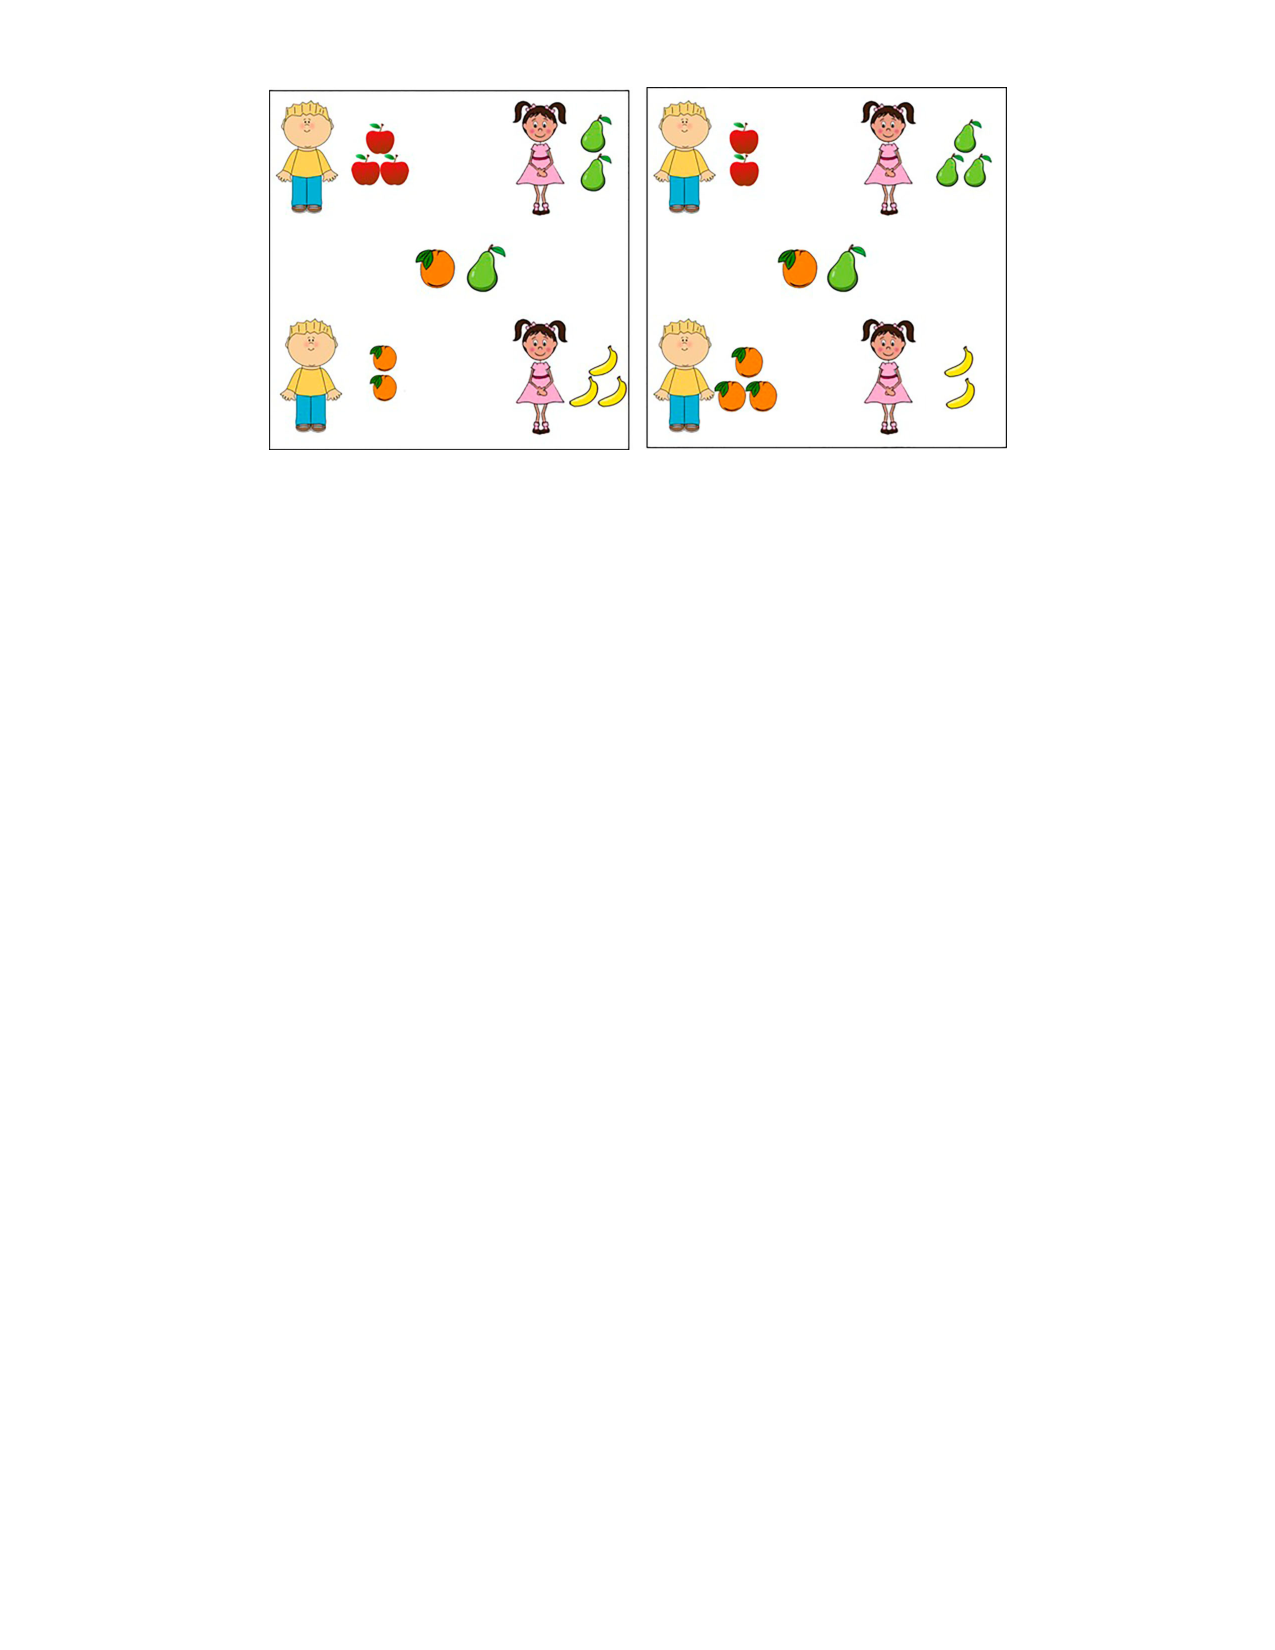
\includegraphics[width=\columnwidth]{images/display}
\caption{Example display from \expref{3} of \citeA{sun2020}. The left image (big \emph{all}/ small  \emph{some}) was paired with  \emph{Click on the boy that has all/three of Susan's apples} or  \emph{Click on the girl that has some/two of Susan's pears}. The right image (small  \emph{all}/ big  \emph{some}) was paired with  \emph{Click on the boy that has all/two of Susan's apples} or  \emph{Click on the girl that has some/three of Susan's pears}.} 
\label{fig:display}
\end{figure}

\begin{figure}
\centering
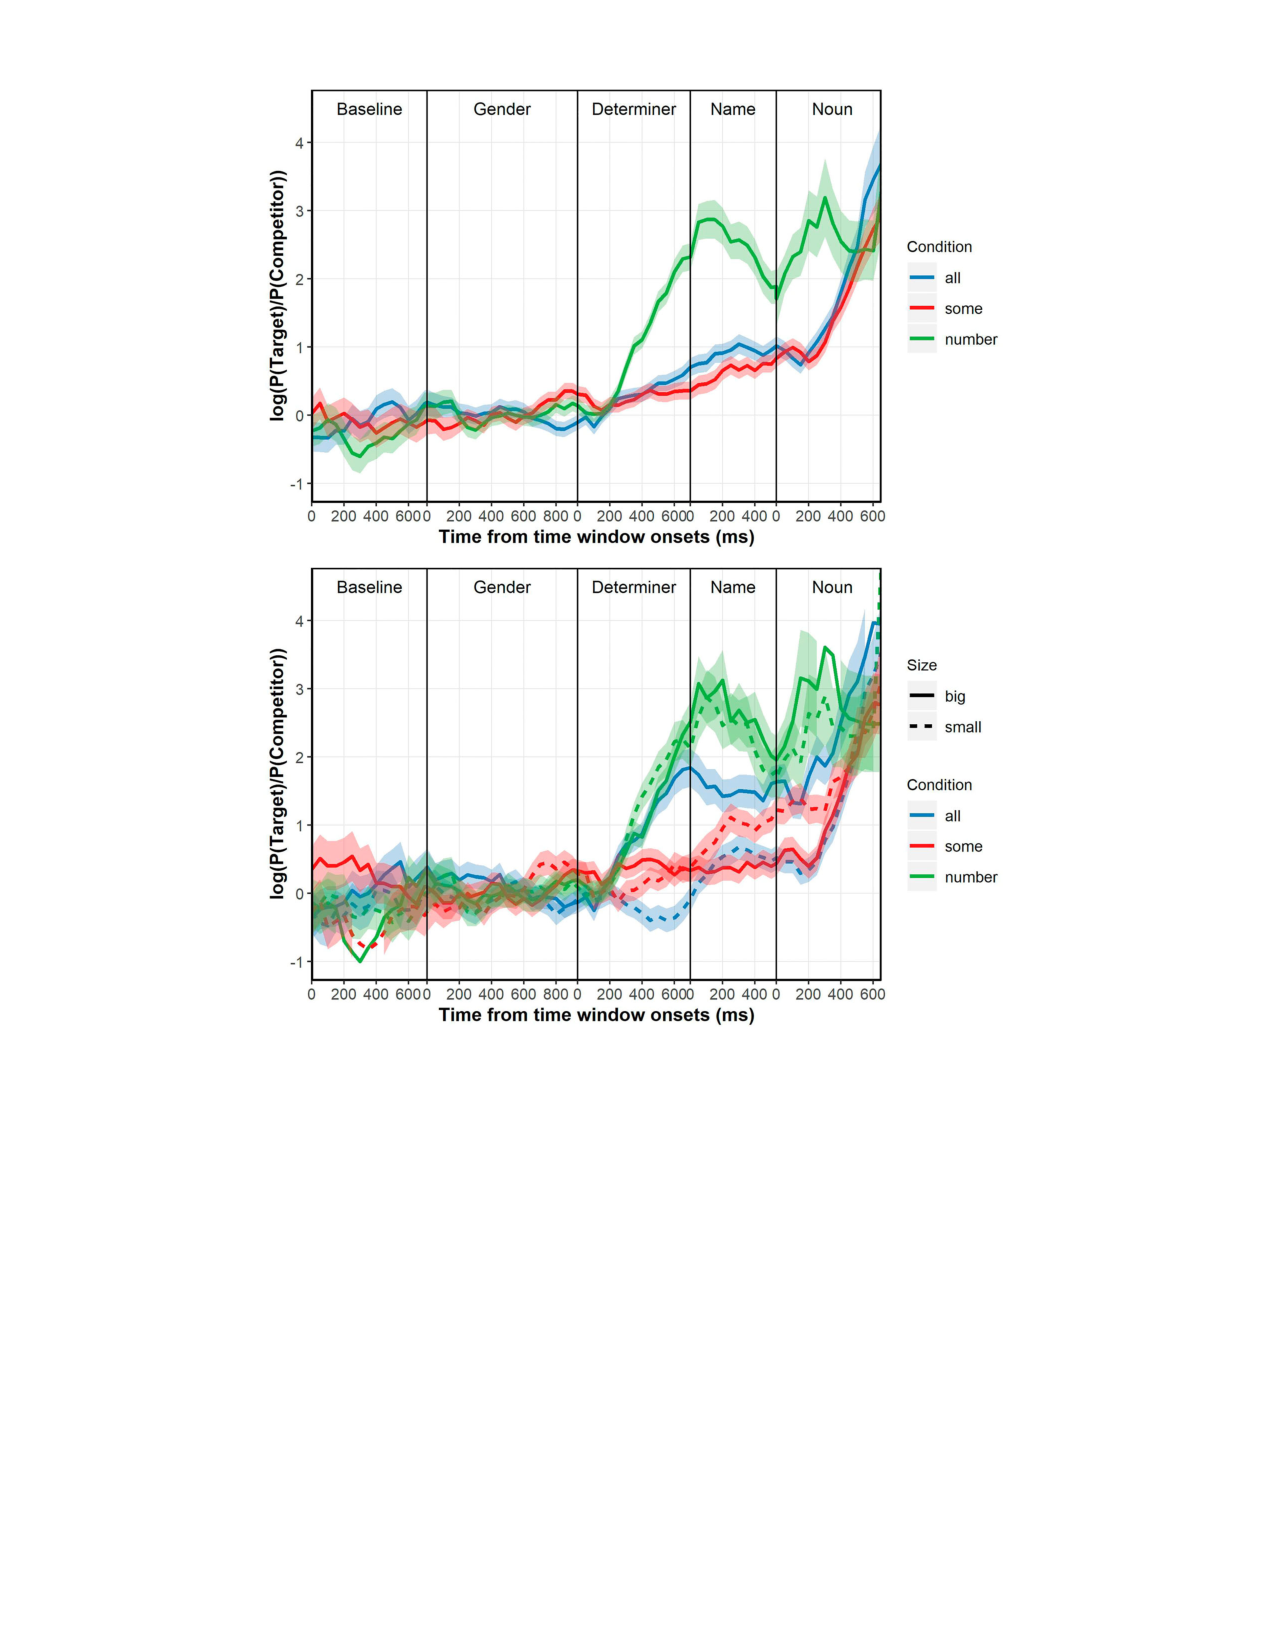
\includegraphics[width=\columnwidth]{images/results-original}
\caption{Eye movement results for \expref{3} of \citeA{sun2020}. Shown are target preference scores from instruction onset to instruction offset. Top: target preference scores by determiner type. Bottom: target preference scores by determiner type and target set size. Transparent ribbons indicate standard error.} 
\label{fig:results-original}
\end{figure}


\section{Exp.~1: replicating Sun \& Breheny (2020) using web-based eye-tracking}

\subsection{Methods}

\textbf{Participants, materials, procedure.}

\subsection{Results}

\section{Exp.~2: replicating Sun \& Breheny (2020) using an incremental decision task}

\subsection{Methods}

\textbf{Participants, materials, procedure.}

\subsection{Results}

The results of a mixed-effects logistic regression in the determiner window, predicting target over competitor choices from fixed effects of quantifier (reference level: ``number"), centered size (higher value: ``big"), and by-item and by-subject random intercepts, and random by-subject slopes from condition and size. There were main effects of condition, such that target selections were less likely in both the \emph{some} ($\beta$=-2.90, $SE$=0.36, $p<$.0001) and \emph{all} ($\beta$=-2.92, $SE$=0.36, $p<$.0001) conditions, compared to the number condition. There was no main effect of size, consistent with the visual result that target selections in the number condition are not modulated by  target set size ($\beta$=-0.09, $SE$=0.26, $p<$.73). However, we did observe interactions between quantifier and size, such that small sets led to more target selections for \emph{some} ($\beta$=0.59, $SE$=0.28, $p<$.05) but to fewer target selections for \emph{all} ($\beta$=-1.27, $SE$=0.29, $p<$.0001), compared to number terms. \jd{does this replicate SB results? also report target preference score analysis?}

%(Intercept)          3.77254    0.39655   9.513  < 2e-16 ***
%conditionall        -2.92409    0.36359  -8.042 8.81e-16 ***
%conditionsome       -2.90211    0.36217  -8.013 1.12e-15 ***
%csize               -0.09207    0.26069  -0.353   0.7239    
%conditionall:csize  -1.27305    0.28523  -4.463 8.08e-06 ***
%conditionsome:csize  0.59465    0.27945   2.128   0.0333 *  

\begin{figure}[H]
\centering
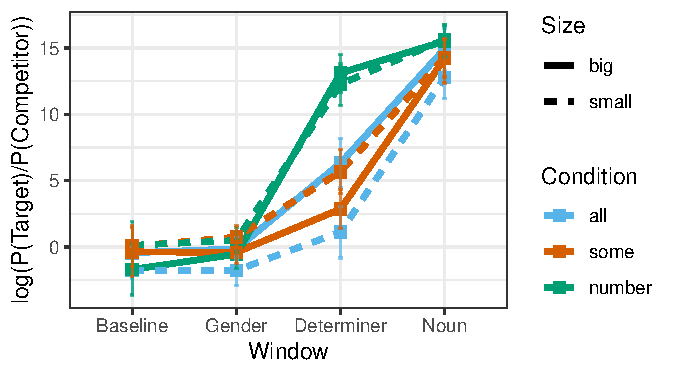
\includegraphics[width=\columnwidth]{../../analysis/SunBreheny/main/graphs/results-idt}
\caption{Proportions of target and competitor selections in Exp.~2 by quantifier and set size.} 
\label{fig:results-idt}
\end{figure}

\section{General discussion}


%\begin{table}[H]
%\begin{center} 
%\caption{Sample table title.} 
%\label{sample-table} 
%\vskip 0.12in
%\begin{tabular}{ll} 
%\hline
%Error type    &  Example \\
%\hline
%Take smaller        &   63 - 44 = 21 \\
%Always borrow~~~~   &   96 - 42 = 34 \\
%0 - N = N           &   70 - 47 = 37 \\
%0 - N = 0           &   70 - 47 = 30 \\
%\hline
%\end{tabular} 
%\end{center} 
%\end{table}


%\begin{figure}[H]
%\begin{center}
%\fbox{CoGNiTiVe ScIeNcE}
%\end{center}
%\caption{This is a figure.} 
%\label{sample-figure}
%\end{figure}


%\section{Acknowledgments}
%
%Madigan, Daisy; chao sun and richard breheny for generously sharing materials, data


\bibliographystyle{apacite}

\setlength{\bibleftmargin}{.125in}
\setlength{\bibindent}{-\bibleftmargin}

\bibliography{sunbrehenyreplication}


\end{document}
